
\documentclass{exam}

\usepackage{graphicx}
\usepackage[fleqn]{amsmath}
\usepackage{unitsdef} 
\usepackage{cancel}
\usepackage{float}
\usepackage{mdwlist}
\usepackage{booktabs}
\usepackage{cancel}
\usepackage{polynom}
\usepackage{caption}
\usepackage{fullpage}
\usepackage{enumerate}

% \newcommand{\degree}{\ensuremath{^\circ}} 
\everymath{\displaystyle}

\newunit{\inch}{in}
\newunit{\foot}{ft}
\newunit{\cemtimeter}{cm}

% \begin{figure}[H]
%   \centering
%   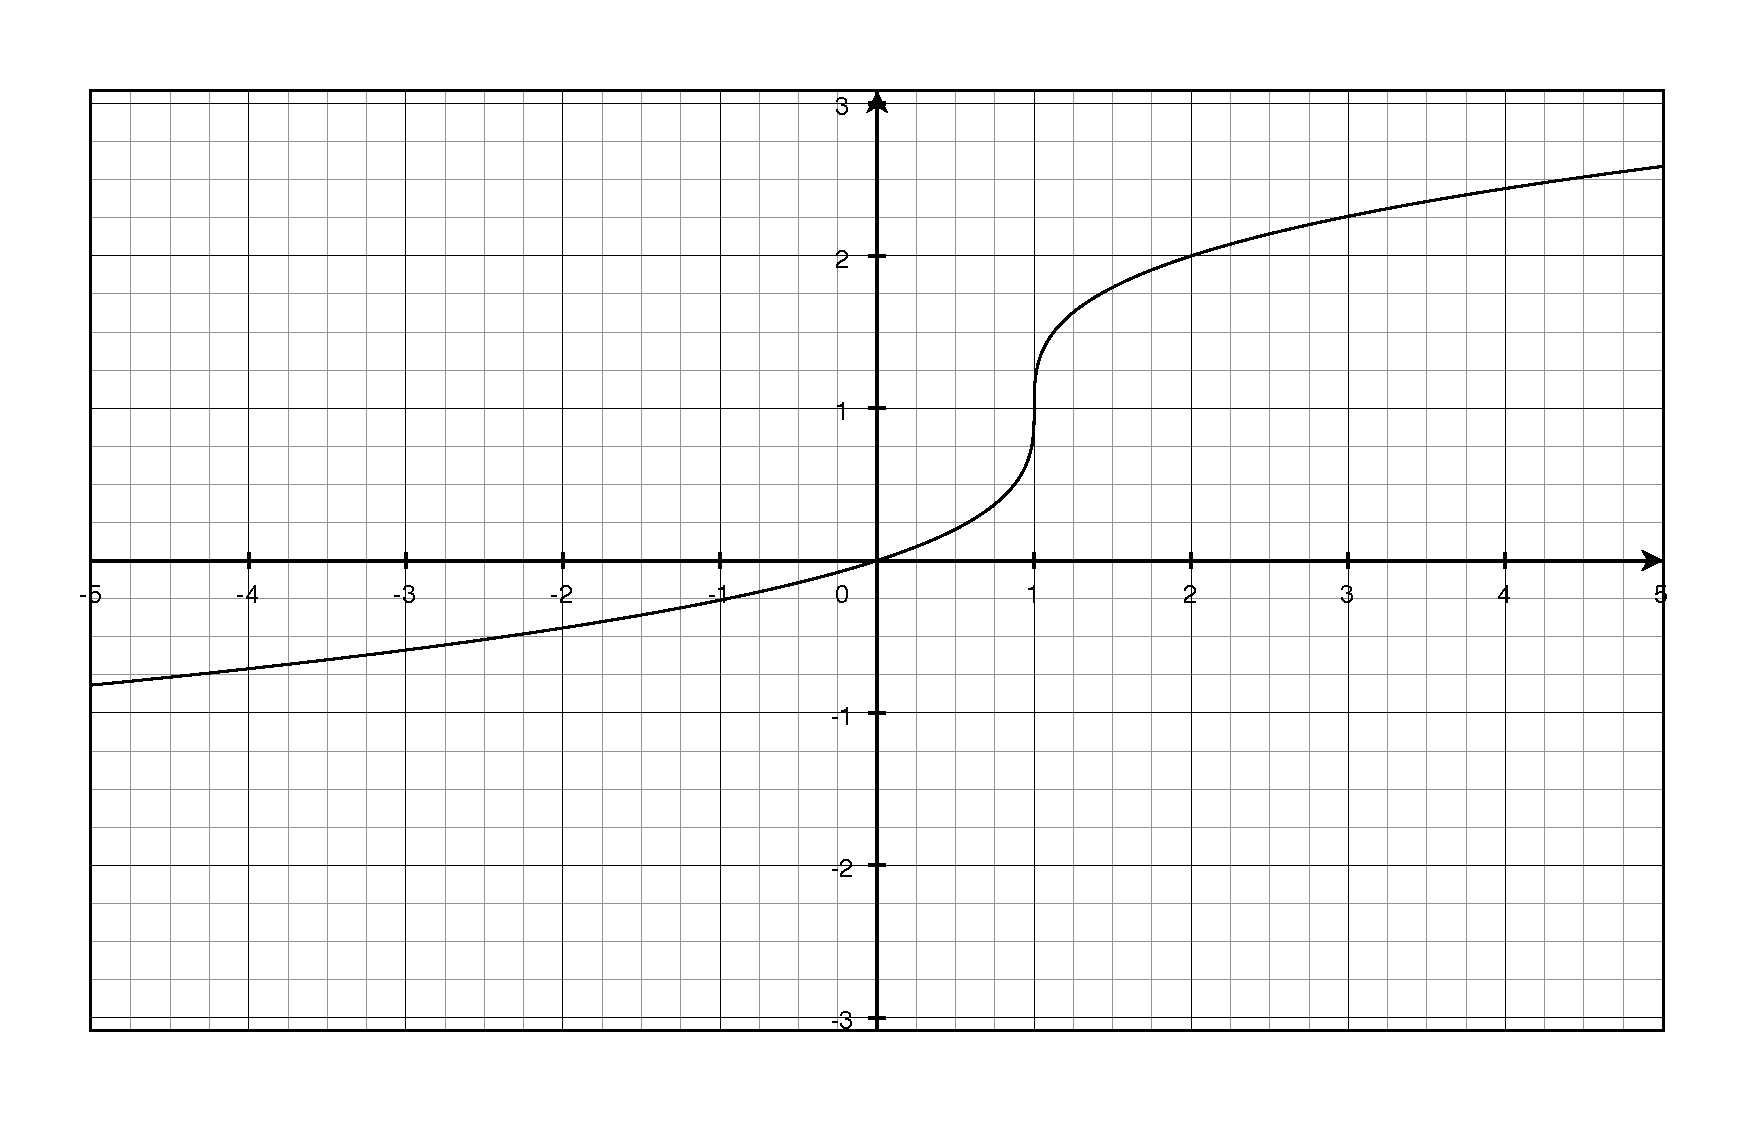
\includegraphics[scale=.3]{question7.eps}
%   \caption*{Question 7}
% \end{figure}

% \begin{tabular}{cc}
% \toprule
% period & amplitude \\
% \midrule
%   $\pi$ & $2$ \\
% \bottomrule
% \end{tabular}

\printanswers

\ifprintanswers 
\usepackage{2in1, lscape} 
\fi

\title{Math 263B \\ Homework Five}
\date{August 9, 2012}

\begin{document}

\maketitle

\section{Homework}

\begin{itemize*}
  \item Read Section 5.7
  \item pp 274-275: 15-19, 25-29, 33-34, 36-40
  \item pp 282-283: 1-17, 20, 24-25, 29-30, 37-41
\end{itemize*}

\section{Extra Credit}
page 283, problem 43

\begin{solution}
From section 5.2, the position function is the antiderivative of the velocity function.
\[
  s(t) = V(t) + C
\]

The total distrance traveled is the difference between the positions at time $a$ and time $b$:
\[
  s_{total} = s(b) - s(a) = V(b) + C - (V(a) + C) = V(b) - V(a)
\]

So the average velocity accoriding to the Section 3.1 definition is:
\[
  v_{avg} = \frac{V(b) - V(a)}{b - a}
\]

The definition of average velocity from this section is:
\[
  v_{avg} = \frac{\int_a^b v \, \mathrm{d}t}{b - a}
\]

According to the Fundamental Theorem of Calculas, this is:
\[
  v_{avg} = \frac{V(b) - V(a)}{b - a} 
\]

and the two definitions match.

\end{solution}

\ifprintanswers

\section{Section 5.6}

\begin{description}

\item[15]

\begin{align*}
  u &= x^2 + 1 \\
  du &= 2x \, dx \\
\\
  \int u^{10} \, \mathrm{d}u &= \frac{1}{11} u^{11} + C \\
  &= \frac{1}{11} (x^2 + 1)^{11} + C \\
\\
  \int_0^1 (x^2 + 1)^{10} (2x) \, \mathrm{d}x &= \frac{1}{11} (x^2 + 1)^{11} \bigg|_0^1 \\
  &= \frac{1}{11} (2^{11} - 1) \\
  &= \frac{2,047}{11} \\
\end{align*}

\item[16]

\begin{align*}
  u &= x^3 + 1 \\
  du &= 3x^2 \, dx \\
\\
  \int u^{1/2} \, \mathrm{d}u &= \frac{2}{3} u^{3/2} + C \\
  &= \frac{2}{3} (x^3 + 1)^{3/2} + C \\
\\
  \int_{-1}^0 (x^3 + 1)^{1/2} (3x^2)  \, \mathrm{d}x &= \frac{2}{3} (x^3 + 1)^{3/2} \bigg|_{-1}^0 \\
  &= \frac{2}{3} \\
\end{align*}

\item[17]

\begin{align*}
  u &= t + 2 \\
  du &= dt \\
\\
  \int u^{-2} \, \mathrm{d}u &= - \frac{1}{u} + C \\
  &= - \frac{1}{t + 2} + C \\
\\
  \int_{-1}^3 \frac{1}{(t + 2)^2} \, \mathrm{d}t &= - \frac{1}{t + 2} \bigg|_{-1}^3 \\
  &= \frac{4}{5} \\
\end{align*}

\item[18]

\begin{align*}
  u &= y - 1 \\
  du &= dy \\
\\
  \int u^{1/2} \, \mathrm{d}u &= \frac{2}{3} u^{3/2} + C \\
  &= \frac{2}{3} (y - 1)^{3/2} + C \\
\\
  \int_{2}^{10} (y - 1)^{1/2} \, \mathrm{d}y &= \frac{2}{3} (y - 1)^{3/2} \bigg|_2^{10} \\
  &= \frac{2}{3} (27 - 1)  \\
  &= \frac{52}{3} \\
\end{align*}

\item[19]

\begin{align*}
  u &= 3x + 1 \\
  dx &= \frac{du}{3} \\
\\
  \int \frac{1}{3} u^{1/2} \, \mathrm{d}u &= \frac{2}{9} u^{3/2} + C \\
  &= \frac{2}{9} (3x + 1)^{3/2} + C \\
\\
  \int_5^8 (3x + 1)^{1/2} \, \mathrm{d}x &= \frac{2}{9} (3x + 1)^{3/2} \bigg|_5^8 \\
  &= \frac{122}{9} \\
\end{align*}

\item[25]
\begin{align*}
  \int_0^{\pi/2} (2x + \sin x) \, \mathrm{d}x &= (x^2 - \cos x) \bigg|_0^{\pi/2} \\
  &= \frac{\pi^2}{4} + 1 \\
\end{align*}

\item[26]
\begin{align*}
  \int_0^{\pi/2} [ 4x + 3 + \cos x) \, \mathrm{d}x &= ( 2x^2 + 3x + \sin x) \bigg|_0^{\pi/2} \\
  &= \frac{\pi^2}{2} + \frac{3 \pi}{2} + 1
\end{align*}

\item[27]
\begin{align*}
  \int_0^4 [x^{1/2} + (2x + 1)^{1/2} \, \mathrm{d}x &= \left( \frac{2}{3} x^{3/2} + \frac{1}{3} (2x + 1)^{3/2} \right) \bigg|_0^4 \\
  &= 14 \\
\end{align*}

\item[28]
\begin{align*}
  \int_{-4}^{-1} \frac{1 - s^4}{2s^2} \, \mathrm{d}s &= \int_{-4}^{-1} \frac{1}{2} (s^{-2} - s^2) \, \mathrm{d}s \\
  &= - \frac{1}{2} \left( \frac{1}{s} + \frac{1}{3} s^3 \right) \bigg|_{-4}^{-1} \\
  &= - \frac{81}{8} \\
\end{align*}

\item[29]
\begin{align*}
  \int_0^1 (x^2 + 2x)^2 \, \mathrm{d}x &= \int_0^1 x^4 + 4x^3 + 4x^2 \, \mathrm{d}x \\
  &= \left( \frac{1}{5} x^5 + x^4 + \frac{4}{3} x^3 \right) \bigg|_0^1 \\
  &= \frac{1}{5} + 1 + \frac{4}{3} \\
  &= \frac{38}{15} \\
\end{align*}

\item[33]
\[
  \int_0^\pi \sin x \, \mathrm{d}x = - \cos x \bigg|_0^\pi = 2
\]

\item[34]
\begin{align*}
  \int_0^1 1 + x + x^2 \, \mathrm{d}x &= \frac{x^2}{2} + \frac{x^3}{3} + x \bigg|_0^2 \\
  &= \frac{40}{3} \\
\end{align*}

\item[36]
\[
  \int_0^1 3 f(x) \, \mathrm{d}x = 3 \int_0^1 f(x) \, \mathrm{d}x = 12
\]

\item[37]
\[
  \int_0^1 [f(x) - g(x) ] \, \mathrm{d}x = \int_0^1 f(x) \, \mathrm{d}x - \int_0^1 g(x) \, \mathrm{d}x = 6
\]

\item[38]
\[
  \int_0^1 [3f(x) + 2 g(x) ] \, \mathrm{d}x = 3 \int_0^1 f(x) \, \mathrm{d}x + 2 \int_0^1 g(x) \, \mathrm{d}x = 8
\]

\item[39]
\[
  \int_0^1 [2g(x) - 3 f(x) ] \, \mathrm{d}x = 2 \int_0^1 g(x) \, \mathrm{d}x - 3 \int_0^1 f(x) \, \mathrm{d}x = -16
\]

\item[40]

\begin{align*}
  \int_1^0 [2f(x) - 3x^2 ] \, \mathrm{d}x &= - \int_0^1 [2f(x) - 3x^2 ] \, \mathrm{d}x \\
  &= - 2 \int_0^1 f(x) \, \mathrm{d}x + \int_0^1 3x^2 \, \mathrm{d}x \\
  &= -8 + x^3 \bigg|_0^1 \\
  &= -7 \\
\end{align*}

  
\end{description}

\section{Section 5.7}

\begin{description}

\item[1]
\[
  \int_1^2 2f(x) \, \mathrm{d}x = 2 \int_1^2 f(x) \, \mathrm{d}x = 6
\]

\item[2]
\[
  \int_0^2 2f(x) \, \mathrm{d}x = 2 \int_0^1 f(x) \, \mathrm{d}x + 2 \int_1^2 f(x) \, \mathrm{d}x = 10
\]

\item[3]
\[
  \int_0^2 [ 2f(x) + g(x) ]\, \mathrm{d}x = 2 \int_0^2  2f(x)\, \mathrm{d}x + \int_0^2 g(x)\, \mathrm{d}x = 14
\]

\item[4]
\[
  \int_0^2 [ 2f(s) + g(s) ]\, \mathrm{d}s = 14
\]

\item[5]
\[
  \int_2^1 [ 2f(x) + 5g(x) ]\, \mathrm{d}x = -2 \int_1^2 f(x) \, \mathrm{d}x - 5 \int_1^2 g(x)  \, \mathrm{d}x = -31
\]

\item[6]
\[
  \int_1^1 [ 3f(x) + 2 g(x) ]\, \mathrm{d}x = 0
\]

\item[7]
\[
  \int_0^2 [ 3f(x) + 2 g(x) ]\, \mathrm{d}x = 3 \int_0^2 f(x) \, \mathrm{d}x + 2 \int_0^2 g(x) \, \mathrm{d}x = 23
\]

\item[8]
\[
  \int_0^2 [ \sqrt{3} f(x) + \sqrt{2} g(x) + \pi]\, \mathrm{d}x = 5 \sqrt{3} + 4 \sqrt{2} + 2 \pi
\]

\item[9]
\[
  \int_0^1 [ f(t) - g(t) + \pi t]\, \mathrm{d}t = 3 + \frac{\pi}{2}
\]

\item[10]
\begin{align*}
  \int_0^1 f(t) \, \mathrm{d}t &+ \int_1^0 t f(t) \, \mathrm{d}t + \int_1^0 \pi g(t) \, \mathrm{d}t \\
  &= - \pi \int_0^1 g(t) \, \mathrm{d}t \\
  &= \pi \\
\end{align*}

\item[11]
\[
  D_x \int_1^x 2t \, \mathrm{d}t = 2x
\]

\item[12]
\[
  D_x \int_x^1 2t \, \mathrm{d}t = - D_x \int_1^x 2t \, \mathrm{d}t = -2x
\]

\item[13]
\[
  D_x \int_0^x (2t^2 + \sqrt{t}) \, \mathrm{d}t = 2x^2 + \sqrt{x}
\]

\item[14]
\[
  D_x \int_0^x \cos^3(2t) \tan(t) \, \mathrm{d}t = \cos^3(2x) \tan(x)
\]

\item[15]
\begin{align*}
  D_x \int_x^{\pi/2} (s - 2) \cot(2s) \, \mathrm{d}s &= - D_x \int_{\pi/2}^x (s - 2) \cot(2s) \, \mathrm{d}s \\
  &= (2 - x) \cot(2x)  \\
\end{align*}

\item[16]
approach 1 (chain rule):
\begin{align*}
  D_x \int_1^x xt \, \mathrm{d}t &= D_x \left( x \cdot \int_1^x t \, \mathrm{d}t \right) \\
  &= x \cdot D_x \left( \cdot \int_1^x t \, \mathrm{d}t \right) + \int_1^x t \, \mathrm{d}t \cdot 1 \\
  &= x \cdot x + \int_1^x t \, \mathrm{d}t \\
  &= \frac{3}{2} x^2 - \frac{1}{2} \\
\end{align*}

approach 2:
\begin{align*}
  \int_1^x xt \, \mathrm{d}t &= \frac{xt^2}{2} \bigg|_1^x \\
  &= \frac{x^3}{3} - \frac{x}{2} \\
\\
  D_x \left( \frac{x^3}{3} - \frac{x}{2} \right) &= \frac{3}{2} x^2 - \frac{1}{2} \\
\end{align*}

\item[17]
\begin{align*}
  u &= x^2 \\
  \frac{du}{dx} &= 2x \\
\\
  D_x \int_1^{x^2} \sin t \, \mathrm{d}t &= \frac{d}{du} \left( \int_1^u \sin t \, \mathrm{d}t \right) \cdot \frac{du}{dx} \\
  &= \sin u \cdot 2x \\
  &= 2x \sin(x^2) \\
\end{align*}


\item[20]
approach 1:
\begin{align*}
  u &= \sin x \\
  w &= \cos x
\\
  D_x \int_{\cos x}^{\sin x} t^5 \, \mathrm{d}t &= D_x \left[ \int_0^{\sin x} t^5 \, \mathrm{d}t - \int_0^{\cos x} t^5 \, \mathrm{d}t \right] \\
  &= \frac{d}{du} \left[ \int_0^u t^5 \, \mathrm{d}t \right] \cdot \frac{du}{dx} - \frac{d}{dw} \left[ \int_0^w t^5 \, \mathrm{d}t \right] \cdot \frac{dw}{dx} \\
  &= u^5 \cos x + w^5 \sin x \\
  &= \sin^5 x \cos x + \cos^5 x \sin x \\
\end{align*}

approach 2:
\begin{align*}
  \int_{\cos x}^{\sin x} t^5 \, \mathrm{d}t &= \frac{1}{6} t^t \bigg|_{\cos x}^{\sin x} \\
   &= \frac{1}{6} (\sin^6 x - \cos^6 x) \\
   D_x \left[ \frac{1}{6} (\sin^6 x - \cos^6 x) \right] &= \sin^5 x \cos x + \cos^5 x \sin x \\
\end{align*}

\item[24]
\begin{align*}
  \int_0^1 1 \, \mathrm{d}x &+ \int_1^2 x \, \mathrm{d}x + \int_2^4 (4 - x) \, \mathrm{d}x \\
  &= x \bigg|_0^1 + \frac{x^2}{2} \bigg|_1^2 + \left(4x - \frac{x^2}{2}\right) \bigg|_2^4  \\
  &= \frac{9}{2} \\
\end{align*}

\item[25]
\begin{align*}
  \int_0^2 (2 - x) \, \mathrm{d}x &+ \int_2^4 (x - 2) \, \mathrm{d}x \\
  &= \left(2x - \frac{x^2}{2} \right) \bigg|_0^2 + \left(\frac{x^2}{2} - 2x \right) \bigg|_2^4 \\
  &= 4 \\
\end{align*}

\item[29]
\begin{align*}
  \int_1^3 4x^3 \, \mathrm{d}x &= x^4 \bigg|_1^3 = 80 \\
  f_{avg} = \frac{80}{2} = 40 \\
\end{align*}

\item[30]
\begin{align*}
  \int_0^3 \frac{x}{\sqrt{x^2 + 16}}\, \mathrm{d}x &= 1 \\
  f_{avg} &= \frac{1}{3} \\
\end{align*}

\item[37]
true.  If $f(x)$ is always positive, than the entire region is above the x axis.

\item[38]
false.  The area of the region above the x axis just has to be larger than the area of the region below the x axis.

\item[39]
false.  The area of the region above the x axis just has to be equal to the area of the region below the x axis.

\item[40]
true.  If there aren't any negative values for $f(x)$, then the only way for the area to be zero is if $f(x)$ is always 0.

\item[41]
true.  Move the right hand integral to the left side and combine.

\end{description}

\else

\vspace{8 cm}

%% The most effective way to restrict democracy is to transfer decision-making from the public arena to unaccountable
%% institutions: kings and princes, priestly castes, military juntas, party dictatorships, or modern corporations.

{In the United States, the political system is a very marginal affair. There are two parties, so-called, but they're
  really factions of the same party, the Business Party. Both represent some range of business interests.}
\vspace{.2 cm}

\hspace{0.5 cm} --Noam Chomsky

%% {\em Some writers have so confounded society with government, as to leave little or no distinction between them; whereas
%%   they are not only different, but have different origins. Society is produced by our wants, and government by our
%%   wickedness; the former promotes our happiness POSITIVELY by uniting our affections, the latter NEGATIVELY by
%%   restraining our vices. The one encourages intercourse, the other creates distinctions. The first a patron, the last a
%%   punisher.} --Thomas Paine

%% {\em I build no system. I ask an end to privilege, the abolition of slavery, equality of rights, and the reign of
%% law. Justice, nothing else; that is the alpha and omega of my argument: to others I leave the business of governing the
%% world.}

%% \vspace{.2 cm}

%% \hspace{1 cm} --Pierre-Joseph Proudhon

\fi

\end{document}

